\section{Funktionsübersicht}
Die verschiedenen Funktionen und deren möglichen Implementierungen sind in
einem morphologischen Kasten zusammengestellt (siehe Tabelle 
\ref{tab:morpho}). In dieser Tabelle sind bereits ausselektierte 
Implementierungen durchstrichen dargestellt. Diese werden aufgrund der
bisherigen Rechercheergebnisse nicht weiter betrachtet.

Die Interpretation des vorliegenden morphologischen Kastens gibt vor, dass
sämtliche Implementierungen als \emph{Module} zu betrachtet sind und sich
gegenseitig nicht ausschliessen oder negativ beeinflussen.

\begin{table}[h!]
	\centering
	\begin{tabular}{l|l l l l l}
		\textbf{Funktion}
			& \textbf{Variante A}
			& \textbf{Variante B}
			& \textbf{Variante C}
			& \textbf{Variante D}
			& \textbf{Variante E} \\
		\hline
		Energieversorgung
			& Akku
			& Druckluft
			& \st{Dampf}
			& Netz
			& \\
		Balllagerung
			& Netz
			& Magazin
			& Korb
			& Rohr
			& \\
		Kommunikation
			& ZigBee
			& Bluetooth
			& WLAN
			& Ad-Hoc
			& \\
		Ortung des Korbes
			& Optik
			& Ultraschall
			& Laser
			& \st{Wärmebild}
			& \st{Radar} \\
		Positionierung
			& fix
			& \st{springt}
			& \st{fliegt}
			& fährt linear
			& \st{rollt} \\
		Balltransport
			& Luft
			& Feder
			& Drehräder
			& Zylinder
			& \\
		Ausrichtung
			& vertikal
			& horizontal
			& 
			&
			& \\
		Externe Steuerungseinheit
			& Notebook
			& Mobile
			&
			&
			& \\
		Bordcomputer
			& Raspberry Pi
			& BeagleBone
			& 
			&
			& \\
	\end{tabular}
	\caption{Morphologischer Kasten der Funktionen}
	\label{tab:morpho}
\end{table}


\subsection{Energieversorgung}

\subsubsection{Akku}

\subsubsection{Drucktank}

\subsubsection{Dampf}

\subsubsection{Netz}

\subsection{2. Ball-Lagerung}

\subsubsection{2.1 Netz}

\subsubsection{2.2 Magazin}

\subsubsection{2.3 Korb}

\subsubsection{2.4 Rohr}

\subsection{Kommunikation}

\subsubsection{ZigBee}

\subsubsection{Bluetooth}

\subsubsection{WLAN (eigenes Netz)}

\subsubsection{WLAN (Ad-hoc)}

\subsection{Externe Steuerungseinheit}
Die externe Steuerungseinheit ist mindestens dafür verantwortlich, dass diese ein Startsignal an die Maschine sendet und am Ende des Vorgangs ein Stoppsignal erhält. Weitere Gedanken gehen dahin, dass die externe Steuerungseinheit aufwändige Berechnungen zur Laufzeit vornehmen kann. Eine zusätzliche Idee ist es, dass diese Einheit Statusmeldungen von der Maschine erhält. Eine Statusmeldung könnte sein "Ortung des Korbes abgeschlossen" oder "Ball 4 abgefeuert".

Ausserdem muss die externe Steuerungseinheit das gewählte Kommunikationsprotokoll unterstützen.

\subsubsection{Notebook}
Ein Notebook als externe Steuerungseinheit ist zu favorisieren. Start-, Stoppsignal und Statusmeldungen zu empfangen sind kein Problem. Zusätzlich bietet heute ein handelsüblicher Notebook bereits sehr viel Rechenpower. Falls die Umsetzung aufwendige Berechnungen erfordert, sollte die Rechenleistung eines modernen Notebooks ausreichen. 

\subsubsection{Mobile}
Mobile steht für ein Smartphone oder auch für ein Tablet. Auch hier sind Start-, Stoppsignal und Statusmeldungen problemlos möglich. Doch diese Variante gilt als "nice-to-have", denn ein solches Geräte verfügt heute noch nicht über die eventuell nötige Rechenleistung eines Notebooks für aufwendige Berechnungen.

\subsection{Ortung des Korbs}
Die Fragestellung lautet: ''Wo ist der Standort des Korbes?''. Um Standorte von Objekten herauszufinden gibt es mehrere Technologien. Die Erkennung hat folgende Herausforderungen:
\begin{itemize}
	\item Distanz 2 Meter
	\item Objekt ist schwarz (guter Kontrast zu Hintergrund)
	\item Beleuchtung nicht konstant
\end{itemize}

\subsubsection{Optik}
Die Umsetzung mittels Optik erfordert auf der Seite der Software-Entwicklung erhöhten Aufwand im Gegensatz zu den anderen Umsetzungsmöglichkeiten. Die Erkennung von Objekten mit einer Kamera hängt zudem stark von den Umgebungsbedingungen ab. Weist ein Objekt z.B. zu wenig Kontrast zu seinem Hintergrund auf wird die Erkennung schwierig. Auch ein Scheinwerfer ist ein möglicher Störfaktor, der zu falschen Messergebnissen führen kann. Diese Probleme können mit einer Justierung der Kamera und der Algorithmen behoben werden. Von den möglichen Störfaktoren abgesehen liefert diese Art der Korbortung sehr präzise Ergebnisse.

Für die Erstellung der Bilder kann eine herkömmliche Webcam verwendet werden. Für den Raspberry Pi wird ausserdem eine günstige und praktische Kamera angeboten. Mittels der Kamera kann ein Bild fotografiert werden, welches ausgewertet wird um den Ort des Korbes zu bestimmen. Geprüft wurden Auswertungsmethoden auf Basis von Java und Python. In beiden Sprachen gibt es mehrere Bibliotheken, welche es erlauben Bildverarbeitung durchzuführen. Im Bereich Java wurde ImageJ (\href{http://imagej.nih.gov/ij/}{http://imagej.nih.gov/ij/}) und in Python wurde OpenCV (\href{http://docs.opencv.org/}{http://docs.opencv.org/}) angeschaut. In beiden Programmiersprachen war es möglich Objekte zu erkennen (siehe Anhang \ref{anhang-bildverarbeitung}).

Eine weitere interessante Lösung für die Objekterkennung ist Pixy. Pixy vereint einen Bildsensor mit einem Prozessor und umgeht so das Problem mit den grossen Datenmengen die ein Bordcomputer (z.B. Raspberry Pi) verarbeiten muss. Zudem sind ist der Bildsensor extrem schnell und hochauflösend. Bei unseren Recherchen hat sich jedoch herausgestellt, dass Pixy mit dem Standartalgorithmus nur farbige Objekt erkennt. Für die Erkennung des Korbes muss der vom Hersteller gelieferte Algorithmus angepasst werden. Die Anpassung ist mit einem gewissen Aufwand und Risiken verbunden und muss gut überlegt werden. Detaillierte Informationen können dem Anhang \ref{anhang-pixy} entnommen werden.

\subsubsection{Ultraschall}
Ultraschall bietet sich an als sehr einfache und preiswerte Technik für ein Ortungssystem.
Verschiedene Tests zeigten, dass typische Ultraschallmodule für die vorgesehene Anwendung
nicht optimal sind (siehe Anhang \ref{sec:hc-sr04}).

\subsubsection{Laser}
Laser- bzw. Infrarotmessmodule bieten sich ähnlich wie Ultraschallmodule als einfache und
preiswerte Ortungssysteme an. Auch hier haben praktische Testst gezeigt, dass einige
Schwierigkeiten auftreten im projektnahen Umfeld \cite{wiki-laser}.

\subsubsection{Wärmebild}
Diese Umsetzung kommt aus mehreren Gründen nicht in Frage. Auf dem Markt gibt es keine Wärmebild Kameras, welche ins Budget passen. Andererseits wird sowohl der Korb wie auch die Wand dahinter dieselbe Wärme aufweisen.

\subsubsection{Radar}

Ein Radargerät sendet elektromagnetische Wellen aus und empfängt das reflektierte Echo. Aus den empfangenen, vom Objekt reflektierten Wellen kann man die Entfernung und die Bewegung eines Objektes bestimmen. Radar erkennt sehr gut Bewegungen auf den Sensor zu. Nicht so gut werden Bewegungen erkannt, die um den Sensor herum geschehen. Auch bei den grossen Elektronikhändler werden nur Bewegungsmelder mit einem Schaltausgang angeboten, der die Position eines Objektes nicht erkennen kann. Deshalb eignet sich die Technologie nicht für die Erkennung des Korbes.


\subsection{6. Positionierung}

\subsubsection{6.1 Fix}

\subsubsection{6.2 Springt in Korb}

\subsubsection{6.4 Fliegen}

\subsubsection{6.5 Geradeaus fahren}

\subsubsection{6.6 Rollt}


\subsection{Balltransport}
Die Bälle müssen die Maschinen mit einer konstanten Geschwindigkeit verlassen und das Ziel möglichst genau treffen. Um die Bälle zu beschleunigen, gibt es verschiedene Möglichkeiten.
\subsubsection{Luft}
Eine Möglichkeit um Bälle zu beschleunigen besteht darin, Druckluft zu verwenden. Die Bälle befinden sich in einer Röhre und werden direkt mit Druckluft beschleunigt. Mit einer präzisen Regulierung des Druckes, der Luft und des Volumenstromes kann die nötige Kraft erreicht werden. Dieses Methode könnte geeignet sein für unseres Projekt.
\subsubsection{Feder}
Die Benutzung der Federn erlaubt ein einfache Berechnung der Kräfte und Energien. Die grösste Schwierigkeit bei der Benutzung der Federn ist die korrekte Wiederpositionierung beim Nachladen, da die Federn sich verbiegen können. Damit das Problem des Nachladens wegfällt, könnten mehrere Abschussrampen gebaut werden.
\subsubsection{Drehräder}
Drehräder sind die am meisten verwendeten Beschleunigungsarten in Ballwerfsystemen. Bei der Benutzung von Drehrädern wird die tangentiale Geschwindigkeit der Drehräder auf den Objekt übertragen. Drehräder können auf verschiedene Arten gebaut werden: zwei Gegenseitige drehende Räder oder ein Rad mit eine Führung.
\subsubsection{Zylinder (Pneumatisch)}
Nach eine vertieften Recherche über die existierenden pneumatische Zylindermodelle, haben wir entschlossen dass kein Zylinder unsere Anforderungen erfüllt. Zudem ergeben sich keine Vorteile gegenüber der Variante mit der Druckluft.  
\subsubsection{Zylinder (Elektromagnetisch)}
Nach einer vertieften Recherche über die existierenden elektromagnetische Zylindermodelle, haben wir entschlossen, dass kein Zylinder unsere Anforderungen erfüllt. Die Modelle die benutzbar wären, brauchen zu viel Energie während einer kurzen Zeitdauer.

\subsection{Ausrichtung}
Um Zeit einzusparen und die Komplexität zu reduzieren, wird die Ballwurfmaschine in der Mitte des Spielfeldes positioniert. Aus diesem Grund muss das Gerät in horizontaler wie auch in vertikaler Richtung ausgerichtet werden können, nachdem der Korb positioniert wurde. 

\subsubsection{horizontale Ausrichtung}
Die horizontale Ausrichtung geschieht mit einem Schrittmotor. Dabei wird der Abwurfmechanismus so ausgerichtet, dass er in Richtung des Korbes zeigt. Um den Abwurfmechanismus und die Kamera miteinander zu verbinden, wird ein Visier vor die Kamera montiert. Das Visier wird auf den Korb ausgerichtet und somit ist auch der Abwurfmechanismus in der richtigen Position zum Abschuss.

\subsubsection{vertikale Ausrichtung}
Damit möglichst wenige Motoren verbaut werden, ist es sinnvoll, die horizontale und vertikale Ausrichtung Mechanisch zu koppeln. Dabei wird die Ballwurfmaschine in horizontaler Richtung mit einem Schrittmotor gedreht. Bei dieser Drehbewegung wird der Abwurfmechanismus über eine Kurvenscheibe geführt, welche den Abschusswinkel einstellt. Dies ist nötig, damit die Tennisbälle mit konstanter Kraft abgeschossen werden können.

\subsection{Bordcomputer}
Die hier als Bordcomputer bezeichnete Komponente steht allgemein für eine
Einheit, welche die \emph{Intelligenz} des Gerätes enthält. Man assoziert
mit dem Bordcomputer geweisse Fähigkeiten wie
\begin{itemize}
	\item Kommunikation (\emph{digitale Datenübertragung})
	\item Aktorenansteuerung
	\item Sensorauswertung
	\item Regelung
\end{itemize}

Die Evaluation eines solchen Bordcomputers kann sehr unterschiedlich 
ausfallen in Abhängigkeit von den gewählten Eigenschaften bzw. 
Ansprüchen an das Gerät. Hier gibt es einige typische Stategien bei der
Auswahl welche je nach Einsatzgebiet gewählt werden.
\begin{description}
	\item[Industrieanwendung] Die Einheit sollte möglichst 
		Einsatzbereit eingekauft werden können und nur eine 
		geringfügige Parametriereung erfordern --- der Preis 
		spielt keine Rolle.
	\item[Massenproduktion] Die Einheit sollte weitestgehend eine
		Eigenentwicklung sein welche genau auf die Aufgaben
		der Applikation zugenschnitten ist --- es muss möglichst
		preiswert sein.
	\item[Einzelanfertigung] Die Einheit sollte möglicht aus 
		gebrauchsfertigen Modulen (Funktionsgruppen) 
		zusammengestellt werden, welche die jeweiligen 
		Anforderungen optimal erfüllen --- es soll schnell zum
		Ziel führen.
\end{description}

Für das vorliegende Projekt ist die dritte Startegie gewählt worden, 
welche sich daran orientiert, möglichst effizient ans Ziel zu gelangen.
Diese \emph{Effizienz} muss für eine konkrete Evaluation jedoch noch
genauer spezifiziert werden. Im vorliegenden Fall ist dies definiert
durch die folgenden Kriterien

\begin{itemize}
	\item Fähigkeiten
	\item Einsatzbereitschaft
	\item Verbreitungsgrad
	\item Leistung
	\item Modifizierbarkeit
	\item Dokumentation
	\item Preis
\end{itemize}

Unabhängig von den oben genannten Kriterien ist auch ein einschneidender
Entscheid getroffen worden, welcher definiert, dass der Boardcomputer
fähig sein muss ein vollwertiges und gängiges Betriebsystem zu 
unterstützen. Dieser Entscheid ist zustande gekommen mit der Absicht, die
Disziplinen Elektrotechnik und Informatik so nahe wie möglich 
zusammenzuführen. Dies vereinfacht die Zusammenarbeit, verhindert 
redundante Arbeitsschritte und erleichtert das Teilen von Ressourcen.
Insbesondere erhofft man sich durch diesen Entscheid eine relevante 
Entlastung der Elektrotechnik, da diese ohnehin mit minimaler Manpower in
der Projektgruppe vertreten ist.

\subsubsection{Raspberry Pi}
Der Raspberry Pi ist ein Einplatinencomputer welcher explizit für
das Experimentieren mit Soft- und Hardware entwickelt worden ist von
der britischen Raspberry Pi Foundation \cite{RPiFoundation}.

Im Gegensatz zu üblichen Computern hat dieser alle für den Betrieb
relevanten Systemkomponenten fix installiert auf einer Platine. Hiervon
ausgenommen ist die Spannungsversogung und der Massenspeicher, welche
jedoch mit gängigen Standards implementiert sind (MicroUSB bzw. MicroSD).

Der Raspberry Pi ist inzwischen sehr weit verbreitet. Dies spiegelt sich
auch wider im grossen Angebot an Literatur, Projekten und Tutorials um
und über den Raspberry Pi.

\begin{figure}[h!]
	\centering
	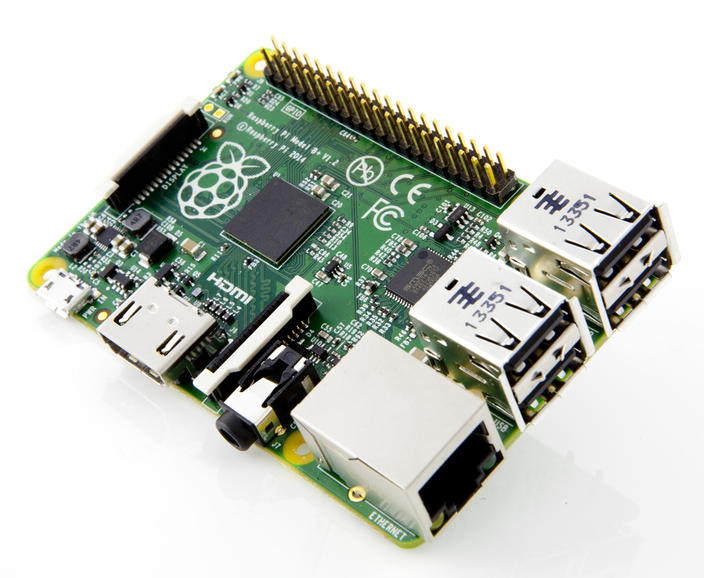
\includegraphics[scale=1]{../../fig/raspberry-pi-b-plus.jpg}
	\caption{Der Rasprberry Pi in der neusten Generation B+ 
		\protect\cite{cnet}}
\end{figure}

Der Raspberry Pi ist als erste Wahl für die Rolle des Bordcomputers 
gewählt worden aufgrund der gegebenen Kriterien, zu denen folgende 
Ergebnisse zustande kamen.

\begin{description}
	\item[Fähigkeiten] Der Raspberry Pi ist in der Lage direkte
		LowLevel Ansteuerung durchzuführen mittels einer Vielzahl
		von Programmiersprachen. Dies ist insbesondere gegeben
		durch die Tatsache, dass ein vollwertiges Betriebsystem
		eingesetzt wird. Durch den Einsatz eines modernen
		Betriebssystems sind auch viele Erweiterungen für Hard- 
		und Software möglich, welche auch auf gewöhnlichen 
		Computern eingesetzt werden. Diese Eigenschaften erfüllen
		das Kriterium der disziplinären Zusammenführung in 
		optimaler Weise.
	\item[Einsatzbereitschaft] Der Raspberry Pi ist ein 
		Einplatinencomputer welcher (ausgehend vom Originalzustand
		wie er vom Hersteller angeboten wird) in wenigen Schritten 
		in Betrieb genommen werden kann. 
	\item[Verbreitungsgrad] Der Raspberry Pi ist einer der
		populärsten Einplatinencomputer mit über 3 Millionen
		verfauften Exemplaren \cite{liz}.
	\item[Leistung] Der Raspberry Pi ist nicht der leistungssrärkste
		Vertreter unter den Einplatinencomputern, bietet dennoch
		gute Kennwerte und besitzt das beste
		Preis-Leistungsverhältnis mit dem geringen Preis \cite{elv}.
	\item[Modifizierbarkeit] Der Raspberry Pi bietet ein vorbereitetes
		Interface an für eine Hardwareerweiterung, welches direkt
		die GPIO und Peripherie-IO zur Verfügung stellt. Auch
		für die Software ist eine hohe Modifizierbarkeit 
		gewährleistet durch den Einsatz von freien und 
		konfigurierbaren GNU/Linux Betriebssystemen.
	\item[Dokumentation] Da der Raspberry Pi explizit zu 
		Bildungs- und Experimentierzwechen entwickelt wurde, 
		bietet der Hersteller auch relevante Daten an für dessen
		Einsatz \cite{RPiSchematics}. Die Entwicklung im Bereich der
		erwerblichen Literatur oder der frei verfügbaren
		Tutorials korreliert mit den Verkaufszahlen und es 
		existieren grosse Benutzergemeindschaften.
	\item[Preis] Die Ziele der Raspberry Pi Foundation bei der
		Entwicklung des Raspberry Pi waren Kompaktheit und ein 
		niedriger Preis \cite{RPiFoundation}. Diese Ziele zeigen sich
		auch im entstandenen Produkt, welches bei offiziellen 
		Distributor für 32.57 SFr. erworben werden kann. Dies ist ein 
		auffallend geringer Preis im Bereich der Einplatinencomputer
		mit ähnlichen Eigenschaften.
\end{description}

Für die Evaluation ist ein aktuelles Modell eines Raspberry Pi mit
ArchLinux aufgesetzt worden. Dieses hat man überprüft auf die 
Lauffähigkeit gewisser Softwarekomponenten und Programmiersprachen,
was bisher positive Ergebnisse geliefert hat. Die bisherigen Ergebnisse
führten zudem zum Fazit, dass der Raspberry Pi ein für die Projektaufgabe
vielseitig einsetzbaren Bordcomputer darstellt, der hinsichtlich seiner
Einsatzfähigkeit nicht weiter untersucht werden muss.

Wie jede andere Komponente eines Systems, kann auch die des Bordcomputers
falsch eingeschätzt werden. Um ein späteres Nachsehen zu vermeiden wird
zu dieser Phase auch gleich evaluiert, wie man kritische Funktionen
aus- bzw. umlagern kann, falls der Raspberry Pi in diesen versagen sollte.

\subsubsection{LowLevel Fallback}
Sollte der Fall eintreten, dass gewisse LowLevel Funktionalitäten nicht
oder nur unter ungünstigen Bedingungen mit dem Raspberry Pi realisiert 
werden können, wird für diese Funktionen ein dediziertes LowLevel 
Mikrocontroller System hinzugezogen. Solche LowLevel Funktionen können
Hardware-Interrupts oder direkte Peripheriekomponenten des Mirkocontrollers
betreffen auf dem auch das Betriebssystem läuft. Diese LowLevel Funktionen
verlangen im Extremfall ein Anpassen des Kernels bzw. das Erstellen eigener
Kernelmodule (Treiberprogramme). Der Overhead, welcher sich beim 
Kerneldevelopment ergeben kann, ist im Verhältnis zum Ergebnis suboptimal. 
Um auf solche Probleme ein Fallback zu haben wird ein einfaches 
Mikrocontrollersystem evaluiert welches ohne Betriebsystem auskommt und
dadurch wesentlich einfacher und dedizierter programmiert werden kann.

\begin{figure}[h!]
	\centering
	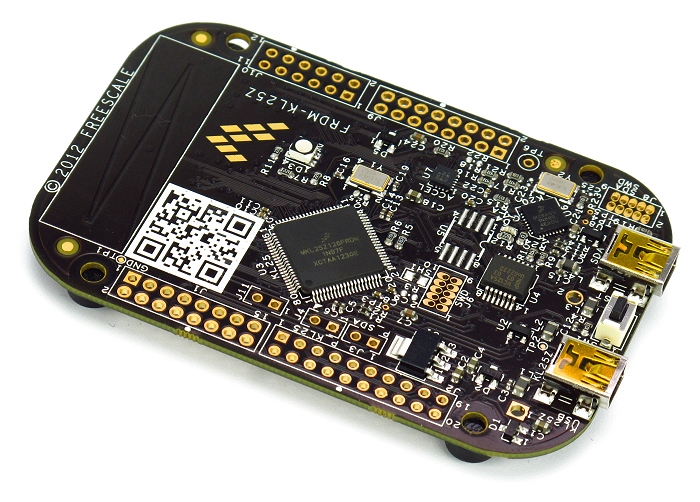
\includegraphics[scale=1]{../../fig/frdm-kl25z.jpg}
	\caption{Das Freedomboard FRDM-KL25Z von Freescale}
\end{figure}

Aktuell wird das Freedomboard FRDM-KL25Z evaluiert. Diese wird im Rahmen
des offiziellen Curriculum der Hochschule Luzern eingesetzt sowie auch
in einem neuen aussercurricularem Kurs für Programmiereinsteiger. Die 
Vorteile, welche sich dadurch ergeben sind erheblich, denn es besteht eine 
grosse Benutzergruppe inklusive Dozenten auf dem Campus Horw welche 
Einführungen, Kursunterlagen und sonstige Informationen und Hilfen anbieten
können. Mit Hilfe dieser Unterlagen war es bereits möglich die Buildutils der 
Hochschule auf Linux zu portieren \cite{ninuxC}. Mit einer Firmware des 
Herstellers und des OpenSDA ist es nun möglich ohne komplizierte Tools eigene
Programme zu entwickeln und zu flashen ohne weitere Geräte. Im Falle eines
plötzlichen Bedarfs für ein Fallback, sind dies entscheidende Kriterien.
Zudem ergibt sich wiederum die vorteilhafte Situation, dass auch die direkte 
Programmierung des Mikrocontrollers von den Informatik-Studenten erfolgen
kann und die geringe Manpower der Elektrotechnik entlastet werden kann
falls dies nötig ist.

\subsubsection{Alternativen}


